\label{chap:differential-evolution}
In the first part of this Chapter we make an overview of the iterative algorithm Differential Evolution, moving later to the mutation and crossover strategies that we have used in the experiments. Finally, we describe DENN (Differential Evolution for Neural Network) - a framework that implements and applies many of the variants, like JADE, SHADE and L-SHADE, of the algorithm Differential Evolution for training ANNs.

% TODO: accenna a DENN e alla sua capacità di allenamento di reti neurali

\section{Differential Evolution}
Differential Evolution (DE) is a metaheuristic\footnote{A metaheuristic is a procedure that has as objective the search, creation or selection of an heuristic that could be find a optimal solution of a problem.} introduced in \cite{DESEHGOCS:1997}, belonging to the family of Evolutionary Algorithms (EAs), that has as objective the searching of a solution through the parallel evolution of a set of candidate solutions.\newline\newline
Differential Evolution is a parallel iterative direct search metaheuristic which utilizes a set, called \textbf{population}, of NP D-dimensional numerical vectors 
\begin{align}
	x_{i},\ i=1,\ \dots,\ NP 
\end{align}
where each of them is called \textbf{individual}, \textbf{genoma} or \textbf{chromosome}. Every individual is manipulated for \textbf{G} generations, where the population is not reduced nor incremented, looking for one individual that can be considered as solution. The search is guided by an objective function called \textbf{fitness function}, which represents the goodness of an individual. For a better research, the individuals should be randomly initialized covering most possible the search space.\newline
\begin{figure}[t]
	\centering
	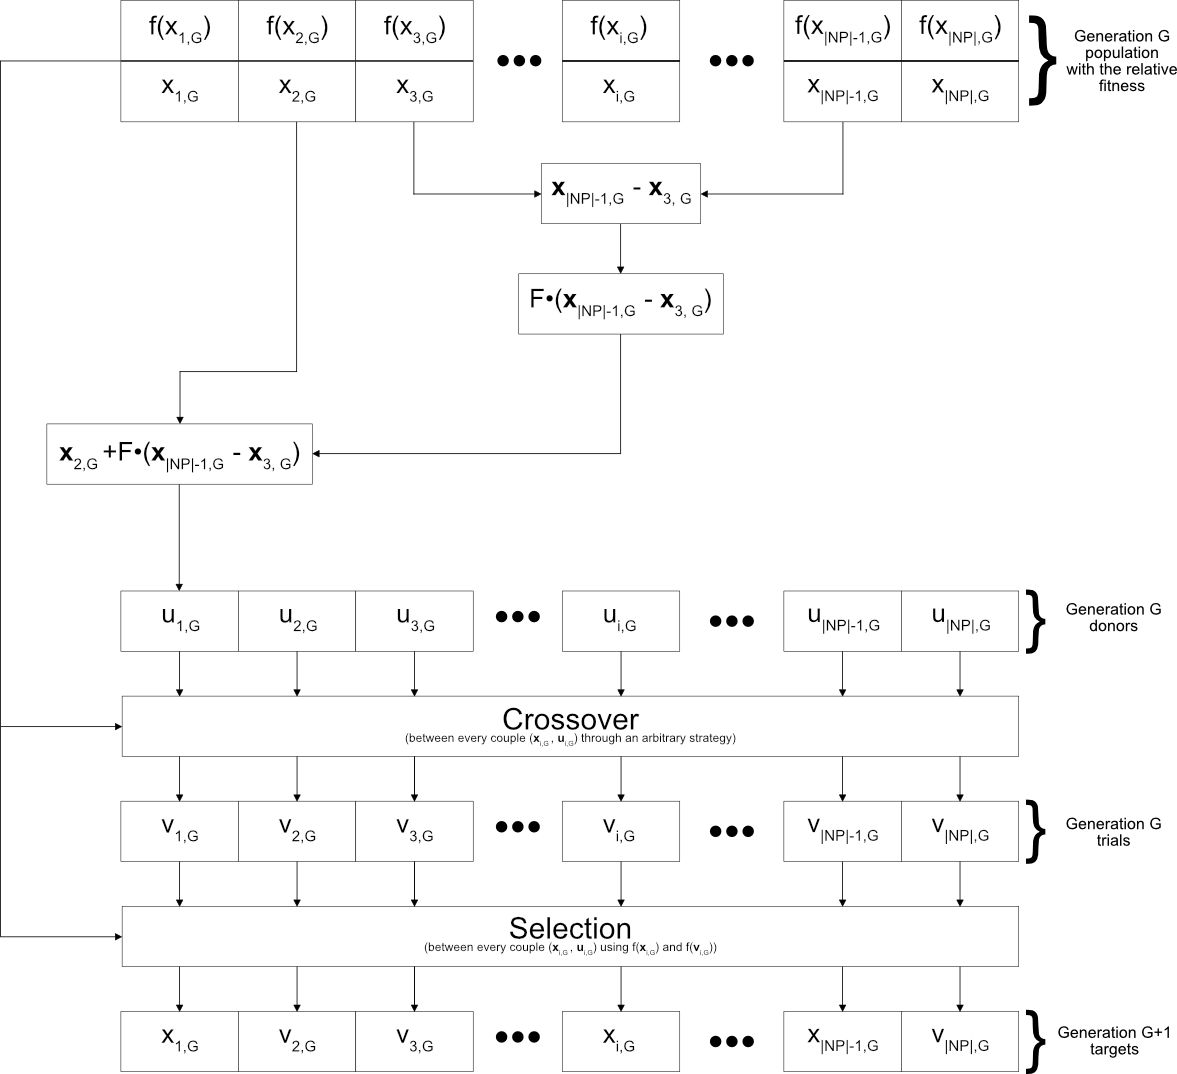
\includegraphics[width=\textwidth]{figures/de-flow-complete.png}
	\caption{Execution flow of the Differential Evolution referred to a generation.}
	\label{fig:bin-crossover}
\end{figure}
In each generation two new sets of individuals are generated, called respectively \textbf{donor} and \textbf{trial} sets. The donors set is generated mixing up individuals, called \textbf{targets}, of the population NP with a mutation operation. The targets and donors are mixed though a crossover method which creates the trials set. After this, the trials is compared one-by-one to the targets with the fitness function - the better are selected creating the targets set of the next generation. \\

\begin{figure}[t]
	\centering
	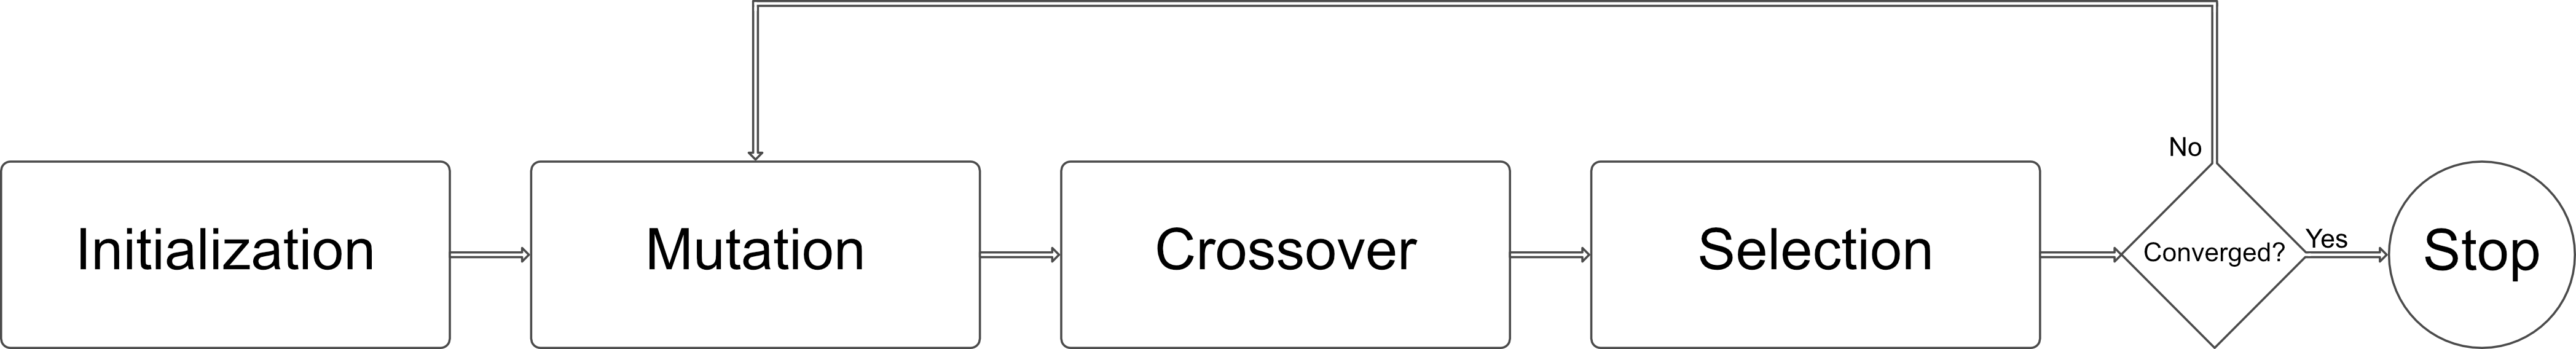
\includegraphics[width=\textwidth]{figures/de-flow.png}
	\caption{Differential Evolution flow diagram.}
\end{figure}

Summing up, firstly the population is initialized with some strategy - the most used is the randomly initialization of each individual. After this step, the operations executed in every DE generation are:
\begin{itemize}
	\item{\textbf{Mutation}: Let $x$ an individual at the generation $G$, also called \textbf{target}. A \textbf{donor} is generated combining $x$ with some other individuals through a differential mutation operation. For example, with the strategy \textbf{rand/1} introduced in \cite{DESEHGOCS:1997} we have
	\begin{align}
		v_{i,G+1} = x_{r_{1},G} + F\cdot(x_{r_{2},G} - x_{x_{3},G})
	\end{align}
	where $r_{1},r_{2},r_{3} \in \{1,2,\dots,NP\}$ are mutually exclusive indices and $F$ is a real-valued constant defined by the user.}
	\item{\textbf{Crossover}: the crossover does nothing else than mixing up one-by-one the donor vectors components with the target vectors with some crossover methods, generating the \textbf{trials} vectors and enhancing the potential diversity of the population. For example, let the target vector $x_{i,G}$ and the mutant $v_{i,G}$ the \textbf{bin} strategy work as follows
\begin{align}
	u_{ji, G} = \begin{cases}
		v_{ji,G}, & \textrm{if}\ (\textit{randb}(j) \leq \textit{CR})\ \textrm{or}\ j=\textit{rnbr}(i)\\
		x_{ji,G}, & \textrm{if}\ (\textit{randb}(j) > \textit{CR})\ \textrm{and}\ j\neq\textit{rnbr(i)}
	\end{cases} & i=1,2,\dots,D
\end{align}
where  $\textit{randb}(j)$ is a function which generate a real valued number for the $j^{th}$ parameter according to binomial distribution, $\textrm{CR}\in[0,1]$ is the global user defined crossover constant used as a threshold and $\textit{rnbr}(i)$ is a function that generate randomly an index which ensures that is selected at least one parameter of the mutant $v_{i}$.}
	\item{\textbf{Selection}: Each trial is compared one-by-one to the corresponding target using the fitness function - if the target have a smaller cost with respect to the trial, than it is retained as individual of the population of the next generation and vice-versa.}
\end{itemize}


\begin{figure}[t!]
	\centering
	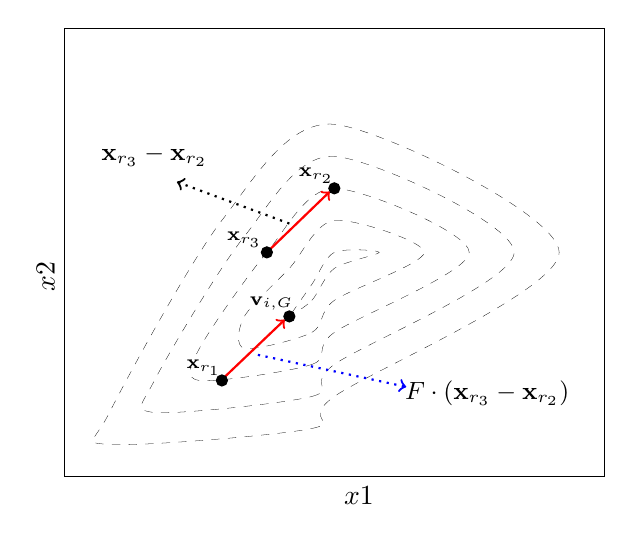
\begin{tikzpicture}[smooth, samples=100]
	
		\begin{axis}[
  			xlabel={$x1$},
  			ylabel={$x2$},
  			xlabel style={below right},
  			ylabel style={above left},
			legend pos=north east,
			ticks=none,
			xmin=5, xmax=65,
			ymin=5, ymax=75
		]
			\addplot[dashed, smooth cycle,ultra thin] coordinates {
    				(30, 30)
    				(32.5, 32.5)
    				(35, 37.5)
    				(40, 40)
    				(35, 40)
    				(32.5, 35)
    				(30, 30)
			};
			
			
			\addplot[dashed, smooth cycle,ultra thin] coordinates {
    				(25, 25)
    				(32.5, 27.5)
    				(35, 32.5)
    				(45, 40)
    				(35, 45)
    				(30, 37.5)
    				(25, 30)
			};
			
			
			\addplot[dashed, smooth cycle,ultra thin] coordinates {
    				(20, 20)
    				(32.5, 22.5)
    				(35, 27.5)
    				(50, 40)
    				(35, 50)
    				(27.5, 40)
    				(20, 25)
			};
			
			
			\addplot[dashed, smooth cycle,ultra thin] coordinates {
    				(15, 15)
    				(32.5, 17.5)
    				(35, 22.5)
    				(55, 40)
    				(35, 55)
    				(25, 42.5)
    				(15, 20)
			};
			
			
			\addplot[dashed, smooth cycle,ultra thin] coordinates {
    				(10, 10)
    				(32.5, 12.5)
    				(35, 17.5)
    				(60, 40)
    				(35, 60)
    				(22.5, 45)
    				(10, 15)
			};
			
			\addplot[only marks] coordinates {
				(27.5, 40)
				(35, 50)
				(22.5, 20)
				(30, 30)
			};
			
			
			\node at (25, 42){\scriptsize $\textbf{x}_{r_3}$};			
			\node at (33, 52){\scriptsize $\textbf{x}_{r_2}$};
			\node at (20.5, 22){\scriptsize $\textbf{x}_{r_1}$};
			\node at (28, 32){\scriptsize $\textbf{v}_{i, G}$};
			
			\node at (axis cs: 15, 55){\small{$\textbf{x}_{r_3} - \textbf{x}_{r_2} $}};
			\node at (axis cs: 52, 18){\small{$F \cdot (\textbf{x}_{r_3} - \textbf{x}_{r_2}) $}};

			\draw[->,red, thick] (27.5, 40) to (34.5, 49.5);
			\draw[->,red, thick] (22.4,20) to (29.5, 29.5);
			\draw[->,dotted,black,thick] (30, 44.5) to (17.5, 51);
			\draw[->,dotted,blue,thick] (26.5,24) to (43,19);
			
			 		
		\end{axis}
	\end{tikzpicture}
	\caption{Illustration of a simple Differential Evolution mutation. $\textbf{v}_{i, G}$ is the new donor vector, created with the scaled difference between $\textbf{x}_{r_2}$ and $\textbf{x}_{r_3}$ combined through summation with $\textbf{x}_{r_1}$.}
	\label{fig:mutant-generation-plot}
\end{figure}

In the algorithm explanation we have described one method for the mutation and one method for the crossover step. Anyway, there exist other methods of mutation and crossover. Hence, in order to classify all the variants the notation $DE/x/y/z$ is used, where:
\begin{itemize}
	\item{\textbf{DE}: indicates the optimization algorithm;}
	\item{\textbf{x}: indicates the mutation strategy;}
	\item{\textbf{y}: indicates how many targets couple are selected in the mutation step;}
	\item{\textbf{z}: indicates the crossover strategy;}
\end{itemize}
Hence, for example, a possible variant is \textit{DE/rand/1/bin}. For the thesis work have been used and tested different configurations of the DE made available by the framework DENN (\ref{sec:DENN}). Hence, about this, following are introduced some of the used algorithms and strategies.
\subsection{Differential Evolution variants}
\subsubsection{Adaptive DE (JADE)}
The base version of Differential Evolution is powerful, but one of its biggest drawback is that the constants $F$ and $CR$ must be selected by the user. Though \cite{RPODE:2005} suggests to set the $F\in[0.4, 0.95]$ and $CR \in (0, 0.2)$, if the function is separable, or $CR \in (0.9, 1.0)$ when the parameters of the function are dependent, this choice remains always a problem dependent decision.Hence, JADE was introduced in \cite{JADE:2009} to solve this problem.\newline\newline
Briefly, this DE variant removes the necessity of selecting the best combination of $F$ and $CR$ constants. This is done with a parameter adaptation system which searches the constants best values refining them at each generation. Moreover, these constants are generated for each individual and so they are, generally, different one from the another, e.g. $\textit{CR}_{1} \neq \textit{CR}_{i}$. Formally what is done is the following:
\begin{itemize}
	\item{\textbf{CR}: Let $\mu_{\textit{CR}}$ be the mean of the $CR$ values, initialized at the first generation to $0.5$. For each generation the crossover probability $\textit{CR}_{i}$ associated to the $x_{i}$ individual, is generated according to a normal distribution with mean $\mu_{CR}$ and a standard deviation $0.1$
	\begin{align}
		\textit{CR}_{i} = \textrm{randn}_{i}(\mu_{\textit{CR}}, 0.1)
	\end{align}
	truncated with respect to the interval $[0, 1]$. \newline\newline
	After each generation, let $S_{CR}$ be the set of the successful $CR$ values, i.e. those values associated to the trials $v$ which are better than the targets $x$. Hence, the mean $\mu_{\textit{CR}}$ is recalculated as follows:
	\begin{align}
		\mu_{\textit{CR}} = (1 - c)\cdot\mu_{\textit{CR}} + c\cdot\textrm{mean}_{A}(S_{\textit{CR}})
	\end{align}
	where the $c\in[0,1]$ is a positive constant  and $mean_{A}(\cdot)$ is the arithmetic mean.	
	}
	\item{\textbf{F}: similarly to CR, \textit{F} is generated for each target with a system similar to that used for CR. Let $\mu_{F}$ the average of the $F$ values, initialized at the first generation to $0.5$. Hence, for each generation and for each target individual,  $F_{i}$ is generated using the mean $\mu_{F}$ and a standard deviation $0.1$ as follows:
		\begin{align}
			F_{i} = \textrm{randc}_{i}(\mu_{F}, 0.1)
		\end{align}
		that is truncated if $F_{i} > 1$ and regenerated if $F_{i} \leq 0$, so that a $F_{i} \in (0, 1]$ and $\textrm{randc}_{i}$ is a Cauchy random generator associated to each target individual.\newline\newline
As for the CR case, let $S_{\textit{F}}$ the set of successful mutation factors to which are added the successful Fs at the end of a generation. Then for each generation the mean $\mu_{F}$ is generated as follows:
		\begin{align}
			\mu_{F} = (1 - c)\cdot\mu_{F} + c\cdot\textrm{mean}_{L}(S_{F})
		\end{align}
		where the $c$ is a positive constant in $[0, 1]$ and $\textit{mean}_{L}$ is the Lehmer mean defined as:
		\begin{align}
			\textrm{mean}_{L}(S_{F}) = \frac{\sum\limits_{F \in S_{F}}F^{2}}{\sum\limits_{F \in S_{F}}F} 
		\end{align}
		}
\end{itemize}

Moreover, JADE has introduced an optional external memory denoted as \textbf{A} with a size equal than \textit{NP}, where all the elements that have failed the selection process is stored. Once the memory is full and it is necessary to add a new failing individual, a randomly selected element is deleted. This optional memory is used in the crossover method named current-to-pbest, as said in Section \ref{subsubsec:curr_p_best}.

\subsubsection{Success-History based Adaptive DE (SHADE)}
The main problem of JADE is that the generation of $\textit{CR}_{i}$ and $F_{i}$ is controlled by the memories $S_{\textit{CR}}$ and $S_{F}$, that for how are managed could contain poor settings of $\textit{CR}$ and $F$. Hence, this fact can leads JADE to have degraded performances.\newline\newline
SHADE introduced in \cite{SHADE:2013} aims to strengthen JADE introducing a crossover and mutation constants generation alternative system. This is done leaving out the $S_{\textit{CR}}$ and $S_{F}$ memories and adding two new memories, named \textit{historical memories}, $M_{\textit{CR}}$ and $M_{F}$ where the values that have well performed in the past are stored.
\begin{table}[t]
	\centering
	\begin{tabular}{|l|l|l|l|l|l|}
		\hline
		Index             & 1                   & 2                   & $\dots$ & $H -1$                & $H$                 \\ 
		\hline
		$M_{\textit{CR}}$ & $M_{\textit{CR},1}$ & $M_{\textit{CR},2}$ & $\dots$ & $M_{\textit{CR},H-1}$ & $M_{\textit{CR},H}$ \\ 
		\hline
		$M_{F}$           & $M_{F, 1}$          & $M_{F, 2}$          & $\dots$ & $M_{F, H-1}$          & $M_{F, H}$          \\ 
		\hline
	\end{tabular}
	\caption{Historical memories $M_{\textit{CR}}$ and $M_{F}$}
\end{table}
Formally, let $M_{F}$ and $M_{\textit{CR}}$ two arrays with $H$ cells all initialized to $0.5$. Similarly to JADE, the constants are generated in each generation for all the individuals like follows:
\begin{align}
	F_i &= \textrm{randc}_{i}(M_{F, r_{i}}, 0.1) \\
	\textit{CR}_i &= \textrm{randn}_{i}(M_{\textit{CR},r_{i}}, 0.1)
\end{align}
where $M_{F, r_{i}}$ and $M_{\textit{CR}, r_{i}}$ are two memory cells randomly selected for each individual. Here the $F_{i}$ and $\textit{CR}_{i}$ are managed like in JADE, i.e. are truncated or regenerated.\newline\newline
In every generation, after the selection is done, the successful $F_{i}$ and $\textit{CR}_{i}$ values are recorded in temporary memories $S_{F}$ and $S_{\textit{CR}}$ with which the content of the memory is updated as follows:
\begin{align}
	M_{F,k,G+1} &= \begin{cases}
		\textrm{mean}_{\textit{WL}}(S_{F}),&\ \textrm{if}\ S_{F} \neq 0 \\
		M_{F,k,G},&\ \textrm{otherwise} \\
	\end{cases}\\
	M_{\textit{CR}, k, G + 1} &= \begin{cases}
		\textrm{mean}_{\textit{WA}}(S_{\textit{CR}}),&\ \textrm{if}\ S_{\textit{CR}} \neq 0 \\
		M_{\textit{CR}},&\ \textrm{otherwise} \\
	\end{cases}
\end{align}
where $k \in [1, H]$ indicates the memory cell to update. k is initialized to 1 and incremented by one at the end of each generation. When $k > H$, is set again to one. Here $\textrm{mean}_{\textit{WL}}$ is the weighted Lehmer mean computed as follows:
\begin{align}
	\textrm{mean}_{\textit{WL}}(S_{F}) &= \frac{\sum_{k=1}^{|S_{F}|}w_{k} \cdot S_{F,k}^2}{\sum_{k=1}^{|S_{F}|}w_{k} \cdot S_{F,k}}
\end{align}
and $\textrm{mean}_{\textit{WA}}$ is the weighted arithmetic mean introduced by Peng et al in \cite{MSJADE:2009}, computed as follows:
\begin{align}
	\textrm{mean}_{\textit{WA}}(S_{\textit{CR}}) &= \sum\limits_{k=1}^{|S_{\textit{CR}}|}w_{k}\cdot S_{\textit{CR},k} \\
	w_k &= \frac{\Delta f_{k}}{\sum_{k=1}^{|S_{\textit{CR}}|}\Delta f_{k}} \\
	\Delta f_{k} &= |f(\textbf{u}_{k,G}) - f(\textbf{x}_{k,G})|
\end{align}
\subsubsection{L-SHADE}
The population size used in a EA algorithm, in this case Differential Evolution, is very important. In fact, a small population results in a faster convergence, but this can also leads the algorithm to fall in a local minimum. Conversely, a larger population increments the algorithm chance to converge to a global minimum by also increasing the computational cost. Hence, the population size is another problem dependent parameter to be optimize.\newline\newline
Hence, to resolve this problem, \cite{LSHADE:2014} introduced L-SHADE, a variant of SHADE that has in addition to $F$ and $\textit{CR}$ constants optimization also a population optimization. This is done through the LSPR (Linear Population Size Reduction), a deterministic linear method that makes a population reduction using a linear function.\newline\newline
Let $\textit{NP}^{\textit{init}}$ the initial population size and $\textit{NP}^{\textit{min}}$ the minimum possible population size to use. Hence, the population for the next generation $G + 1$ is calculated as follows:
\begin{equation}
	\textit{NP}_{G + 1} = \textrm{round}\Bigg[\Bigg(\frac{\textit{NP}^{\textit{min}} - \textit{NP}^{\textit{init}}}{\textit{MAX\_NFE}} \Bigg) \cdot \textit{NFE} + \textit{NP}^{\textit{init}} \Bigg]
\end{equation}
where \textit{NFE} is the current number of fitness evaluations and \textit{MAX\_NFE} is the maximum number of fitness evaluations. The linear function at the time of population generation is not constrained to the previous population, so if $\textit{NP}_{G + 1} > \textit{NP}_{G}$ then the worst $(\textit{NP}_{G} - \textit{NP}_{G+1})$ individuals are pruned from the population having also in this case a linear population reduction.
\subsection{Mutation strategies}

\subsubsection{Rand}
The Rand mutation strategy is introduced in \cite{DESEHGOCS:1997} and works selecting randomly the individuals with which the donors/mutant is created. The procedure is as follows:
\begin{align}
	v_{i, G + 1} &= x_{r_{1}} + F \cdot (x_{r_2, G} - x_{r_3, G}) \\
	v_{i, G + 1} &= x_{r_{1}} + F \cdot (x_{r_2, G} - x_{r_3, G}) + F \cdot (x_{r_4, G} - x_{r_5, G})
\end{align}
where $r_1, r_2, r_3, r_4, r_5 \in \{1, 2, \dots, \textit{NP}\ \}$ must be mutually different and also from the related index $i$.

\subsubsection{Best}
The Best mutation strategy is introduced in \cite{DESEHGOCS:1997} and works selecting, as the name suggests, the current best individual and some other as follows:
\begin{align}
	v_{i, G + 1} &= x_{\textit{best}, G} + F \cdot (x_{r_1, G} - x_{r_2, G}) \\
	v_{i, G + 1} &= x_{\textit{best}, G} + F \cdot (x_{r_1, G} + x_{r_2, G} - x_{r_3, G} - x_{r_4, G})
\end{align}
where, as for rand, $r_1, r_2, r_3, r_4 \in \{1, 2, \dots, \textit{NP}\ \}$ must be mutually different and also from the related index $i$.

\subsubsection{DEGL}
Differently from the previous two methods, DEGL, introduced in \cite{DEGL:2009}, makes a topological neighborhood exploration, i.e. for each generation, DEGL, creates every individuals $\textbf{v}_{i, G + 1}$ belonging to the donors set through a convex combination between the local mutant $\textbf{L}_{i, G}$ and the global mutant $\textbf{g}_{i, G}$.\newline\newline
Formally, let the $\textit{NP}_G$ population at generation G, disposed with a ring topology. For each individual $\textbf{x}_{i, G}$ is a neighborhood defined of $k \in [0, (\textit{NP} - 1) / 2]$ individuals, consisting in vectors $\textbf{x}_{i - k, G}, \dots, \textbf{x}_{i + k, G}$. 
For each individual $\textbf{x}_{i, G}$ a local mutant $\textbf{L}_{i, G}$ and a global mutant $\textbf{g}_{i, G}$ are created as follows:
\begin{align}
	\textbf{L}_{i, G} &= \textbf{x}_{i, G} + \alpha \cdot (\textbf{x}_{\textit{n\_best}_i, G} - \textbf{x}_{i, G}) + \beta \cdot (\textbf{x}_{p, G} - \textbf{x}_{q, G}) \\
	\textbf{g}_{i, G} &= \textbf{x}_{i, G} + \alpha \cdot (\textbf{x}_{\textit{g\_best}, G} - \textbf{x}_{i, G}) + \beta \cdot (\textbf{x}_{r_1, G} - \textbf{x}_{r_2, G})
\end{align}
where $\textit{n\_best}_i$ indicates the best individual in the neighbors of $\textbf{x}_{i, G}$ differently to $\textit{g\_best}$ which is the global best individual, $p, q \in [i - k, i + k]$, with $p \neq q \neq i$, and $r_1, r_2 \in NP_{G}$, with $r_1 \neq r_2 \neq i$. $\alpha$ and the $\beta$ are real-valued scalar used as scaling factors.\newline\newline
After the creation of local and global donor vectors, each of them are combined through convex combination using a scalar weight $w \in (0, 1)$ in the following mode:
\begin{equation}
	\textbf{V}_{i, G} = w \cdot \textbf{g}_{i, G} + (1 - w) \cdot \textbf{L}_{i, G}
\end{equation}

\subsubsection{Current-to-pbest}\label{subsubsec:curr_p_best}
Current to pbest is introduced in \cite{JADE:2009} as an evolution of best method. In fact, best is a greedy strategy which uses prevalently the information of the best solution and this could lead the search to converge to local minimum. Instead in current-to-pbest this information can impact partially on the search, reducing in this way the possibility that the search algorithm stops in a local minimum.\newline\newline
This strategy exists in two versions which differentiate in the use of an auxiliary memory. The base version does not use the auxiliary memory and creates each donor $\textbf{u}_{i, G}$ as follows:
\begin{equation}
	\textbf{u}_{i, G} = \textbf{x}_{i, G} + F_i \cdot (\textbf{x}_{\textit{best}, G}^p - \textbf{x}_{i, G}) + F_i \cdot (\textbf{x}_{r_1, G} - \textbf{x}_{r_2, G})
\end{equation}\label{eqn:curr_p_best}
where $\textbf{x}_{\textit{best}, G}$ is an individual chosen among the $100p\%$ of the current population $\textit{NP}_{G}$ and $F_i$ is the mutation factor which is associated to every individual and managed as in JADE and SHADE.\newline\newline
Denoting by \textbf{A} the auxiliary memory where are stored the elements that have failed the selection process (e.g. if $f(\textbf{x}_{i, G}) < f(\textbf{v}_{i, G})$, then $\textbf{x}_{i, G}$ is added to $\textbf{A}$), the alternative version of Current to pbest with memory works as follows:
\begin{equation}
	\textbf{u}_{i, G} = \textbf{x}_{i, G} + F_i \cdot (\textbf{x}_{\textit{best}, G}^{p} - \textbf{x}_{i, G}) + F_i \cdot (\textbf{x}_{r_1, G} - \tilde{\textbf{x}}_{r_2, G})
\end{equation}
where $\textbf{x}_{\textit{best}, G}$, $\textbf{x}_{r_1, G}$ and $\textbf{x}_{i, G}$ are selected as in \ref{eqn:curr_p_best} and $\tilde{\textbf{x}}_{r_2, G}$ is selected, instead, in $\textbf{P} \cup \textbf{A}$. Note that if $\textbf{A}$ size exceeds a certain threshold, then some solutions are randomly removed.\newline\newline
The Current-to-pbest is further improved in association with SHADE. Here, the constant $p$ existing in JADE versions is substituted with a variable version, i.e. to each individuals a value $p_i$ is associated as follows:
\begin{equation}
p_i = rand[p_{\textit{min}}, 0.2]
\end{equation}
where $p_{\textit{min}} = 2 / \textit{NP}_G$, so that at least 2 individuals are selected, and 0.2 is the maximum value as suggest in \cite{JADE:2009}.
\subsection{Crossover strategies}

\subsubsection{Bin}
\begin{figure}[h]
	\centering
	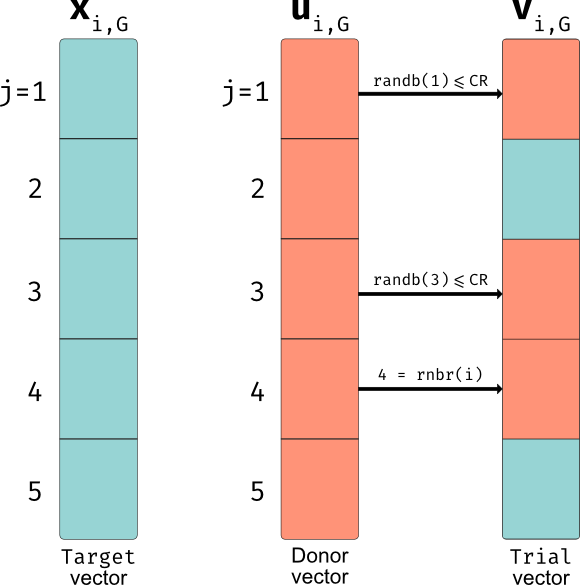
\includegraphics[width=0.4\textwidth]{figures/de-rand.png}
	\caption{Bin crossover strategy illustration with $D = 5$.}
	\label{fig:bin-crossover}
\end{figure}

Bin is classic form of crossover and works as follows:
\begin{equation}
	u_{ij, G} = \begin{cases}
		v_{ij, G}, &\textrm{if }\textit{randb}(j) \leq \textit{CR}\textrm{ or } j = \textit{rnbr}(i)\\
		x_{ij, G}, &\textrm{otherwise}
	\end{cases}
\end{equation}
where $\textit{randb}(i) \in [0, 1]$ is a uniform random generator and $\textit{rnbr}(j) \in [1, D]$ so that at least one component of mutant $\textbf{v}_{i, G}$. The figure \ref{fig:bin-crossover} gives a visual representation of the strategy.

\subsubsection{Exp}
\begin{figure}[h!]
	\centering
	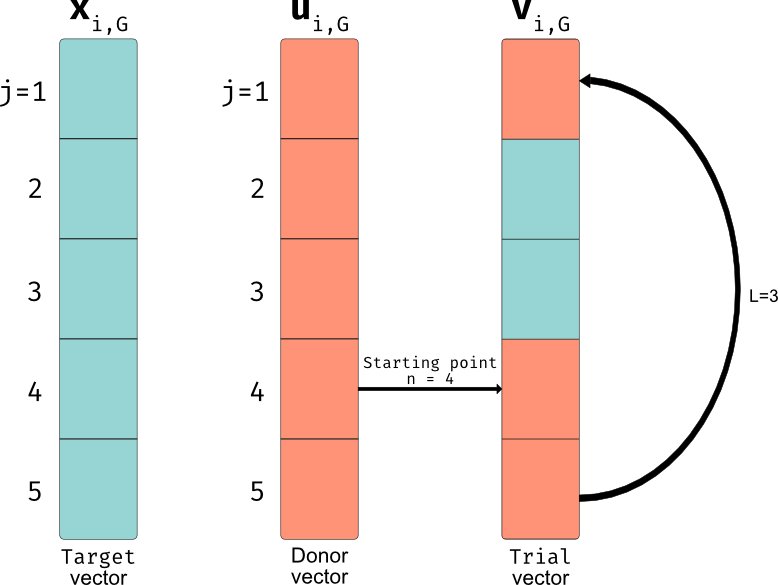
\includegraphics[width=0.5\textwidth]{figures/de-exp.png}
	\caption{Exp crossover strategy illustration with a $N = 4$ as starting point and $L = 3$ parameters to substitute.}
	\label{fig:exp-crossover}
\end{figure}
The crossover Exp, starts by choosing a random $n \in [1, D]$, used as an initial point in the target value where the parameters substitution starts, and a integer $L \in [1, D]$ that represents the parameters to substitute. So after choosing this two values, a trial vector is created as follows:
\begin{align}
	v_{ij, G} &= u_{ij, G}\textrm{,  for } j = \{<n>_{D}, \dots, <n + L - 1>_{D}\} \\
	v_{ij, G} &= x_{ij, G}\textrm{,  otherwise}
\end{align} 
where $< \cdot >_{D}$ is the modulo function with modulus D. An example is showed in figure \ref{fig:exp-crossover}

\section{DENN}\label{sec:DENN}
DENN is a framework written in C++ by Gabriele Di Bari and Mirco Tracolli, based on their thesis work. It aims to apply the Differential Evolution concepts on the ANN training as an alternative to Gradient-based algorithms. It has been initially created as a TensorFlow extension due to the performance and simplicity offered by this latter, but now it is completely based on the C++ library Eigen due to its implementation based on the high performance library LAPACK written in Fortran 77.

\subsection{How it works}
DENN is a framework that aims to help the developer to construct a system to train Neural Networks with Differential Evolution. To achieve this goal, DENN is structured in pluggable modules through which is decided how the neural network should be trained. For example, let the Differential Evolution configuration JADE/\\Rand/1/Bin - JADE, Rand/1 and Bin are three modules that can be selected for the training process at the time of configuration of DENN. The plug-in that could be used are not only for the DE, but also regard the dataset\footnote{Where is it, how to manage it, etc.}, how the neural network should be structured\footnote{How many levels and the activation functions} and, more important, what kind of neural network you want instruct\footnote{At this time, DENN can trains only feed-forward networks.}. Some of the configuration parameters can be found in the Table \ref{tbl:denn-parameters}.\newline\newline
As said in the Chapter \ref{chap:differential-evolution}, Differential Evolution bases its functioning also on the existence of a population of vectors, called \textit{NP}, that is parallel evolved by the optimization algorithm aiming to arrive to the fitness function minimum value, i.e. to a solution vector which has the fitness minimum value. By the definition of DE, it is assumed that vectors are multi-dimensional, i.e. a list of features to optimize. Hence in DENN, since the population is composed by neural networks it cannot be used as is, instead the individuals must be managed as a set of weights and biases matrices, i.e. every individual is a neural network and is formed by a weights and biases matrices set. Hence, the mutation and crossover actions are not executed over the whole structure of individuals, but singularly over their subcomponents.\newline\newline
For a better explanation, let's examine the mutation phase through an example. Let \textit{NP} the Neural Networks population, Rand/1 the mutation strategy, $r_1, r_2$ and $r_3$ three mutually exclusive indexes, the donor $\textbf{u}_{1}$ is created as follows:
\begin{align}
	\textbf{u}_{1}^{w_1} &= \textbf{x}_{r_1}^{w_1} + F \cdot (\textbf{x}_{r_2}^{w_1} - \textbf{x}_{r_3}^{w_1}) \\
	\textbf{u}_{1}^{b_1} &= \textbf{x}_{r_1}^{b_1} + F \cdot (\textbf{x}_{r_2}^{b_1} - \textbf{x}_{r_3}^{b_1}) \\
	\cdots \cr
	\textbf{u}_{1}^{w_{|\textbf{HL}|}} &= \textbf{x}_{r_1}^{w_{|\textbf{HL}|}} + F \cdot (\textbf{x}_{r_2}^{w_{|\textbf{HL}|}} - \textbf{x}_{r_3}^{w_{|\textbf{HL}|}}) \\
	\textbf{u}_{1}^{b_{|\textbf{HL}|}} &= \textbf{x}_{r_1}^{b_{|\textbf{HL}|}} + F \cdot (\textbf{x}_{r_2}^{b_{|\textbf{HL}|}} - \textbf{x}_{r_3}^{b_{|\textbf{HL}|}})
\end{align}
where $w_i$ and $b_i$ represent the weights and bias vectors of the $\textrm{i}^{\textrm{th}}$ level and \textbf{HL} is the hidden layers set. The same work is made also for the crossover phase, so we do not explain it with an example which is leaved to the reader.

\begin{table}[]
	\centering	
	\begin{tabular}{|l|l|}
		\hline
		\rowcolor{Gray}Argument     & Description \\ \hline

		\rowcolor{LightGray}\multicolumn{2}{|c|}{\textbf{Execution args}} \\ \hline
		threads\_pop & Executed threads of DENN \\ \hline
		seed     	 & Distribution seed \\ \hline
		instance		 & Type of model (nram/default) \\ \hline \hline

		\rowcolor{LightGray}\multicolumn{2}{|c|}{\textbf{Batch info}} \\ \hline
		batch\_size  	 & Number of training examples \\ \hline
		batch\_offset	 & Examples per batch \\ \hline
		use\_validation & Activate pop validation at the end of a sub-		geneneration \\ \hline
		cumpte\_test\_per\_pass     	 & Compute the test accuracy for each pass \\ \hline \hline

		\rowcolor{LightGray}\multicolumn{2}{|c|}{\textbf{DE}} \\ \hline
		generations  	 & Total number of generations \\ \hline
		sub\_gens  	 	& Number of sub-generations \\ \hline
		number\_parents  	 	& DE population size \\ \hline
		f						& DE F coefficient \\ \hline
		cr						& DE CR coefficient \\ \hline
		evolution\_method 		& Evolution method (JADE/SHADE/L-SHADE) \\ 	\hline
		mutation 				& Mutation method (degl/curr\_p\_best) \\ \hline
		crossover				& Crossover method (bin/exp/interm) \\ \hline \hline

		\rowcolor{LightGray}\multicolumn{2}{|c|}{\textbf{Network}} \\ \hline
		hidden\_layers  	 		& Levels size \\ \hline
		activation\_functions  	& Activation functions of levels \\ \hline \hline

		\rowcolor{LightGray}\multicolumn{2}{|c|}{\textbf{NRAM}} \\ \hline
		task  	 		& Task to execute \\ \hline
		max\_int  		& Max int in the set \\ \hline
		sequence\_size  & The size of the input sequence \\ \hline
		n\_registers  	& Registers to use \\ \hline
		time\_steps  	& Execution timesteps \\ \hline
		gates  			& Gates to use \\ \hline
		change\_difficulty\_level & The lambda under of which the difficulty can be changed \\ \hline
		step\_gen\_change\_difficulty & Number of gen where the same difficulty is used  \\ \hline

	\end{tabular}
	\caption{Some arguments could be used in the configuration file of DENN.}
	\label{tbl:denn-parameters}
\end{table}